\documentclass[12pt]{extarticle}
%Some packages I commonly use.
\usepackage[english]{babel}
\usepackage{graphicx}
\usepackage{framed}
\usepackage[normalem]{ulem}
\usepackage{amsmath}
\usepackage{amsthm}
\usepackage{amssymb}
\usepackage{amsfonts}
\usepackage{enumerate}
\usepackage[utf8]{inputenc}
\usepackage{float}
\usepackage[top=1 in,bottom=1in, left=1 in, right=1 in]{geometry}

%A bunch of definitions that make my life easier
\newcommand{\matlab}{{\sc Matlab} }
\newcommand{\cvec}[1]{{\mathbf #1}}
\newcommand{\rvec}[1]{\vec{\mathbf #1}}
\newcommand{\ihat}{\hat{\textbf{\i}}}
\newcommand{\jhat}{\hat{\textbf{\j}}}
\newcommand{\khat}{\hat{\textbf{k}}}
\newcommand{\minor}{{\rm minor}}
\newcommand{\trace}{{\rm trace}}
\newcommand{\spn}{{\rm Span}}
\newcommand{\rem}{{\rm rem}}
\newcommand{\ran}{{\rm range}}
\newcommand{\range}{{\rm range}}
\newcommand{\mdiv}{{\rm div}}
\newcommand{\proj}{{\rm proj}}
\newcommand{\R}{\mathbb{R}}
\newcommand{\N}{\mathbb{N}}
\newcommand{\Q}{\mathbb{Q}}
\newcommand{\Z}{\mathbb{Z}}
\newcommand{\<}{\langle}
\renewcommand{\>}{\rangle}
\renewcommand{\emptyset}{\varnothing}
\newcommand{\attn}[1]{\textbf{#1}}
\theoremstyle{definition}
\newtheorem{theorem}{Theorem}
\newtheorem{corollary}{Corollary}
\newtheorem*{definition}{Definition}
\newtheorem*{example}{Example}
\newtheorem*{note}{Note}
\newtheorem{exercise}{Exercise}
\newcommand{\bproof}{\bigskip {\bf Proof. }}
\newcommand{\eproof}{\hfill\qedsymbol}
\newcommand{\Disp}{\displaystyle}
\newcommand{\qe}{\hfill\(\bigtriangledown\)}
\setlength{\columnseprule}{1 pt}

\usepackage{xcolor}

\usepackage{gensymb}
\definecolor{myBlue}{RGB}{0,133,255}%{HTML}{0085ff}
\usepackage{tikz}
\newcommand\phase[1]{\tikz[baseline=(X.base)]\node [draw=myBlue,fill=myBlue,thick,rectangle,inner sep=2pt, rounded corners=2pt](X){\color{white}\textbf{#1}};}




\usepackage{hyperref}

\title{\textbf{SOCRaTEs}\\
\textbf{S}imulink \textbf{O}racles for \textbf{C}PS \textbf{R}equiremen\textbf{T}s\\ with unc\textbf{E}rtainty}
\author{Menghi Claudio, Nejati Shiva,  Khouloud Gaaloul,  Lionel Briand}
%\date{January 2019}
\date{\vspace{-5ex}}

%\geometry{paperwidth=170mm, paperheight=16383pt, left=40pt, top=40pt, textwidth=280pt, marginparsep=20pt, marginparwidth=100pt, textheight=16263pt, footskip=40pt}

\begin{document}

\maketitle

\vspace{1cm}
\begin{itemize}
\item Section~Overview provides an overview on SOCRaTEs.
\item Section~Installation and Project Creation describes how to install SOCRaTEs and how to create your first SOCRaTEs project.
\item Section~Using SOCRaTEs describes how to use SOCRaTEs.
\item Finally Section~Tutorial provides a  tutorial that describes how to use SOCRaTEs on a set of simple examples.
\end{itemize}





\section{Overview}
Figure~1 shows an overview of SOCRaTeS (\emph{Simulink Oracles for CPS RequiremenTs with uncErtainty}),  our approach to generate automated test oracles for CPS models.  SOCRaTeS takes three inputs: (\phase{1}) a CPS model with parameters or inputs involving uncertainties, (\phase{2}) a set of functional requirements for the CPS model and (\phase{3}) a set of test inputs that are developed by engineers to test the CPS model with respects to its requirements. 
SOCRaTeS makes  the following assumptions about its inputs:

\begin{itemize}
\item \emph{The CPS model is described in Simulink} (\phase{1}). Simulink allows specifying dynamic systems, it is executable and allows engineers to test their models as early as possible.  
\item \emph{Functional requirements are described in a signal logic-based language} (\phase{2}).  
We present our requirements language later in this document.
\item \emph{A set of test inputs exercising requirements are provided} (\phase{3}).
We assume engineers have a set of test inputs for their CPS model. The test inputs may be generated manually, randomly or based on any test generation framework proposed in the literature. SOCRaTeS is agnostic to the selected test generation method. 
\end{itemize}



SOCRaTeS automatically converts functional requirements into oracles specified in Simulink (\phase{4}). The oracles evaluate test outputs of the CPS model in an automated and online manner and generate fitness values that provide engineers with a degree of satisfaction or failure for each test input (\phase{5}). Engineers can stop running a test in the middle when SOCRaTeS concludes that the test fitness is going to  remain below a given threshold for the rest of its execution. 


\begin{figure}
\caption{An Overview on SOCRaTEs.}
  \centering
    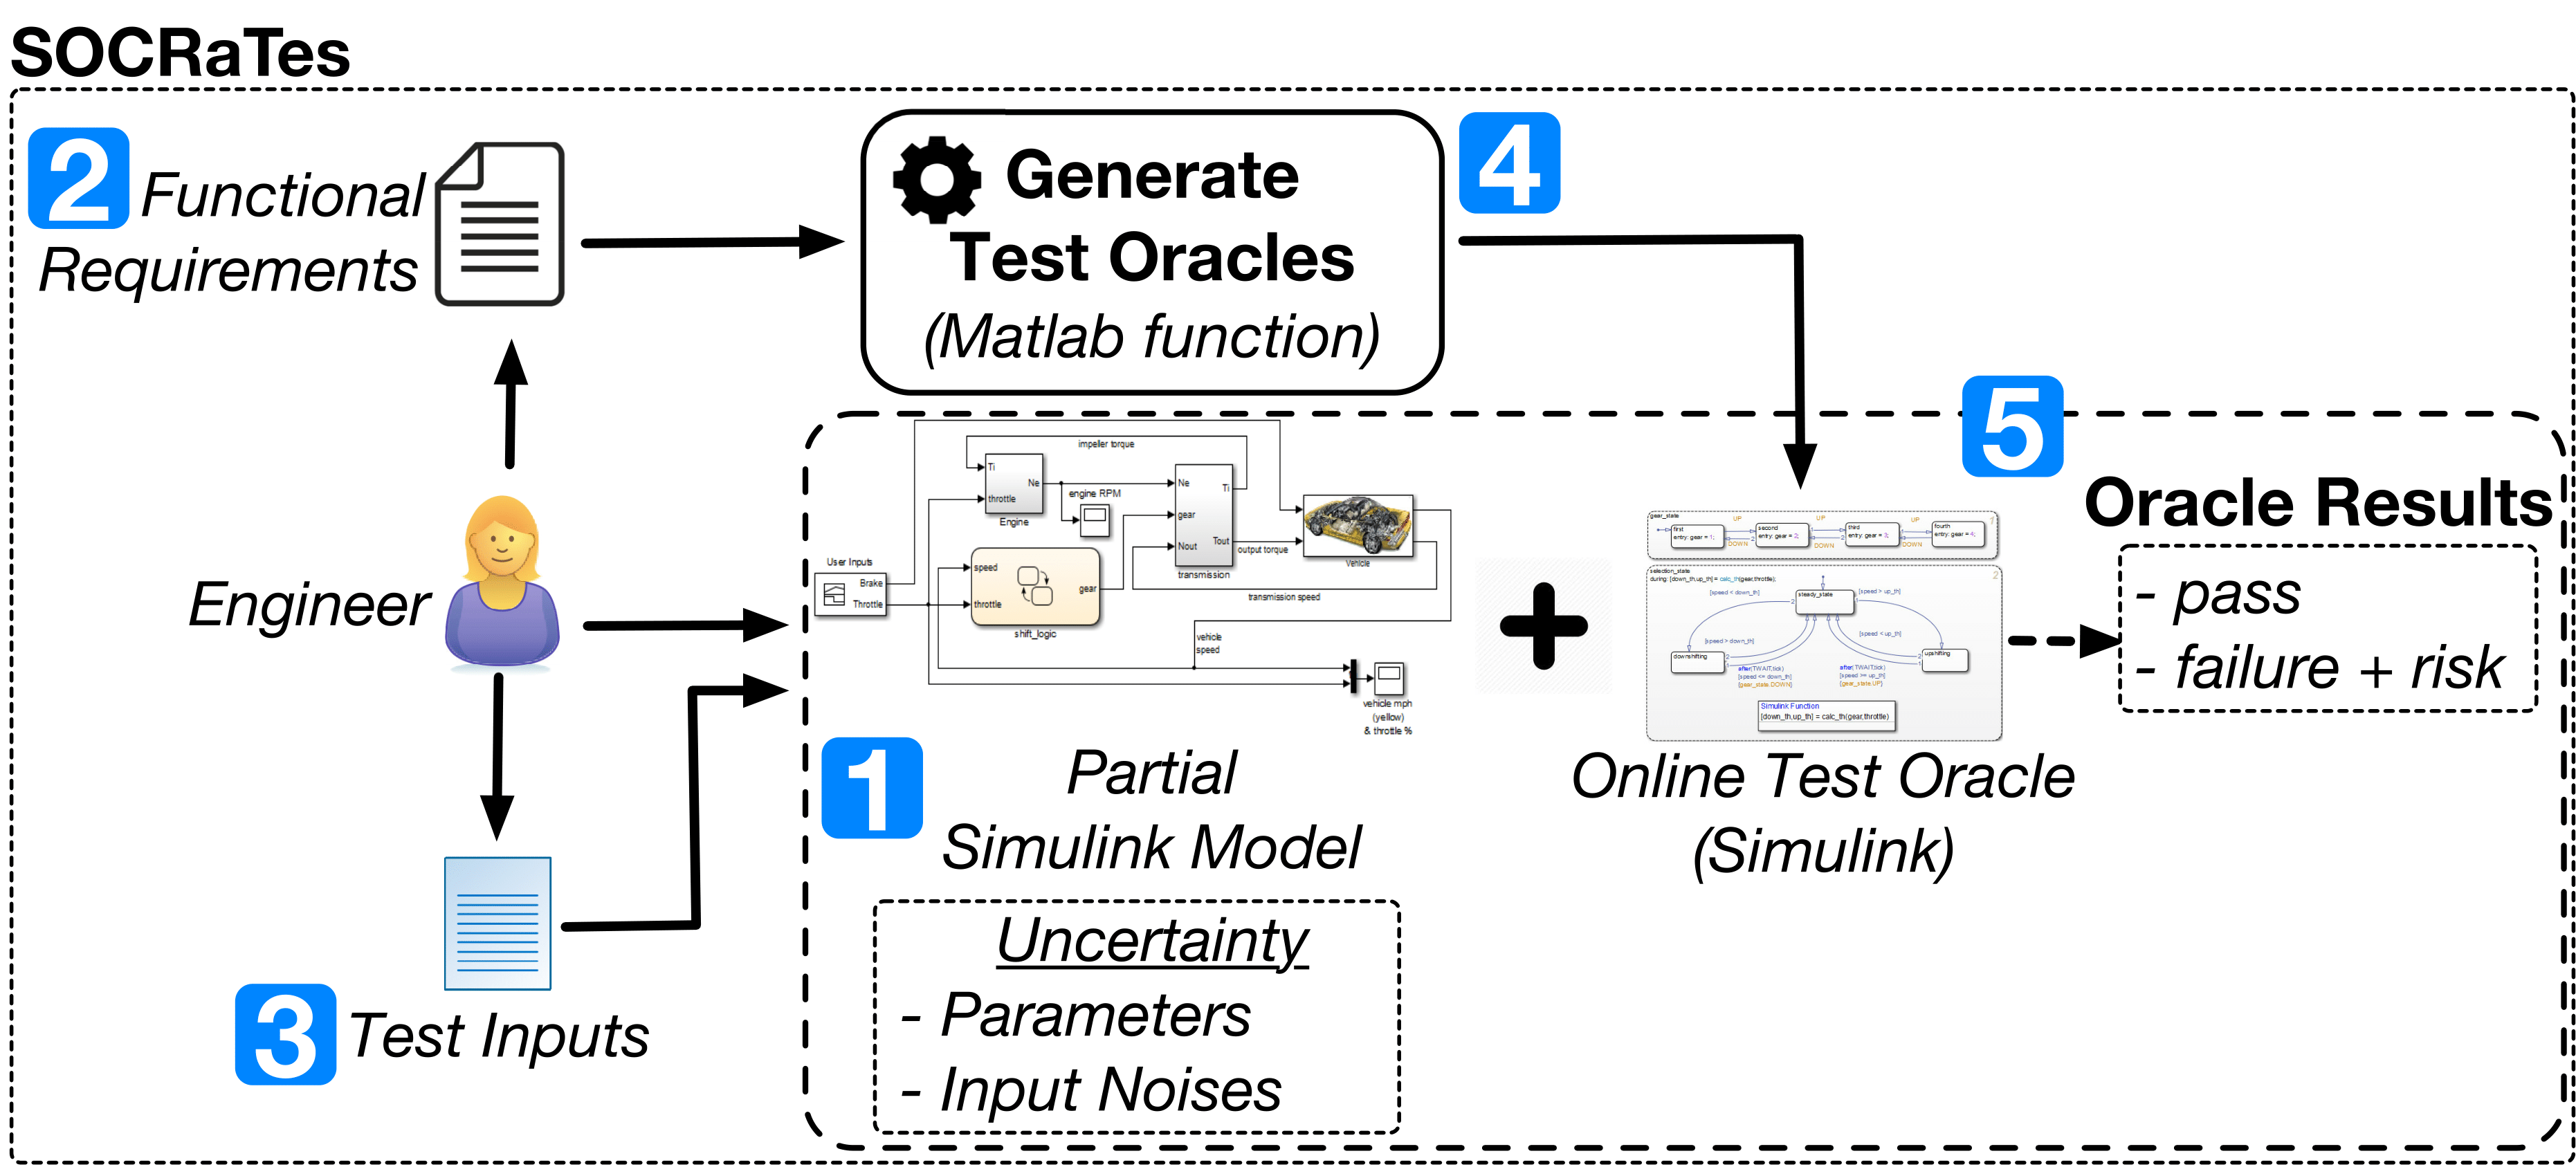
\includegraphics[width=0.7\textwidth]{Manual/Overview.png}
\end{figure}

\section{Installation and Project Creation}

\subsection{Prerequisite}
The following software must be installed on your laptop to run Socrates
\begin{itemize}
\item Eclipse (\url{https://www.eclipse.org/})
\item Java 1.8 or superior
\item Matlab/Simulink
\end{itemize}

\subsection{Installing Socrates}
Socrates can be installed by performing the following steps:
\begin{itemize}
\item Click on Help $>$ Install new Software $>$ Add $>$ Local
\item Select the Plugin folder;
\item Uncheck Group items by category;
\item Select Socrates SDK feature;
\item Click on Next $>$ Next $>$ I accept $>$ Finish.
\end{itemize}

\subsection{Creating a New Project}
To create a new project perform the following steps:
\begin{itemize}
\item File $>$ New $>$ Project;
\item Select Project from General;
\item Click on Finish;
\end{itemize}


\section{Using SOCRaTEs}

\subsection{Creating a your Requirements}
\begin{itemize}
\item Create a file .socrates (File $>$ New $>$ File);
\item When asked to convert into an Xtext project click on Yes.
\end{itemize}

\subsection{Generating the .m files using Socrates}
\begin{itemize}
\item copy the file demo.socrates within your workspace.
\item Change the file (e.g., add a new blank line) and save it
\item	When you save the file a file .m is automatically created in the folder src-gen/ModelName.
\end{itemize}

\subsection{Adding the oracles into your model}
\begin{itemize}
\item	Open the Simulink model test
\item	Copy the file Test\_Req.m into your workspace
\item	Run Test\_Req in Matlab
\item	tollerableriskTest\_Req=0;
\item	Run your simulation
\end{itemize}


\clearpage
\section{Tutorial}
We consider four different scenarios obtained by considering two different models and two requirements.

\subsection{The Considered Models}
The first model generates a sine wave with amplitude $2$ and frequency $1$ $rad/s$ that is represented in Figure~2.

\begin{figure}[h]
\caption{The signal $e$ generated from the model Model 1.}
  \centering
    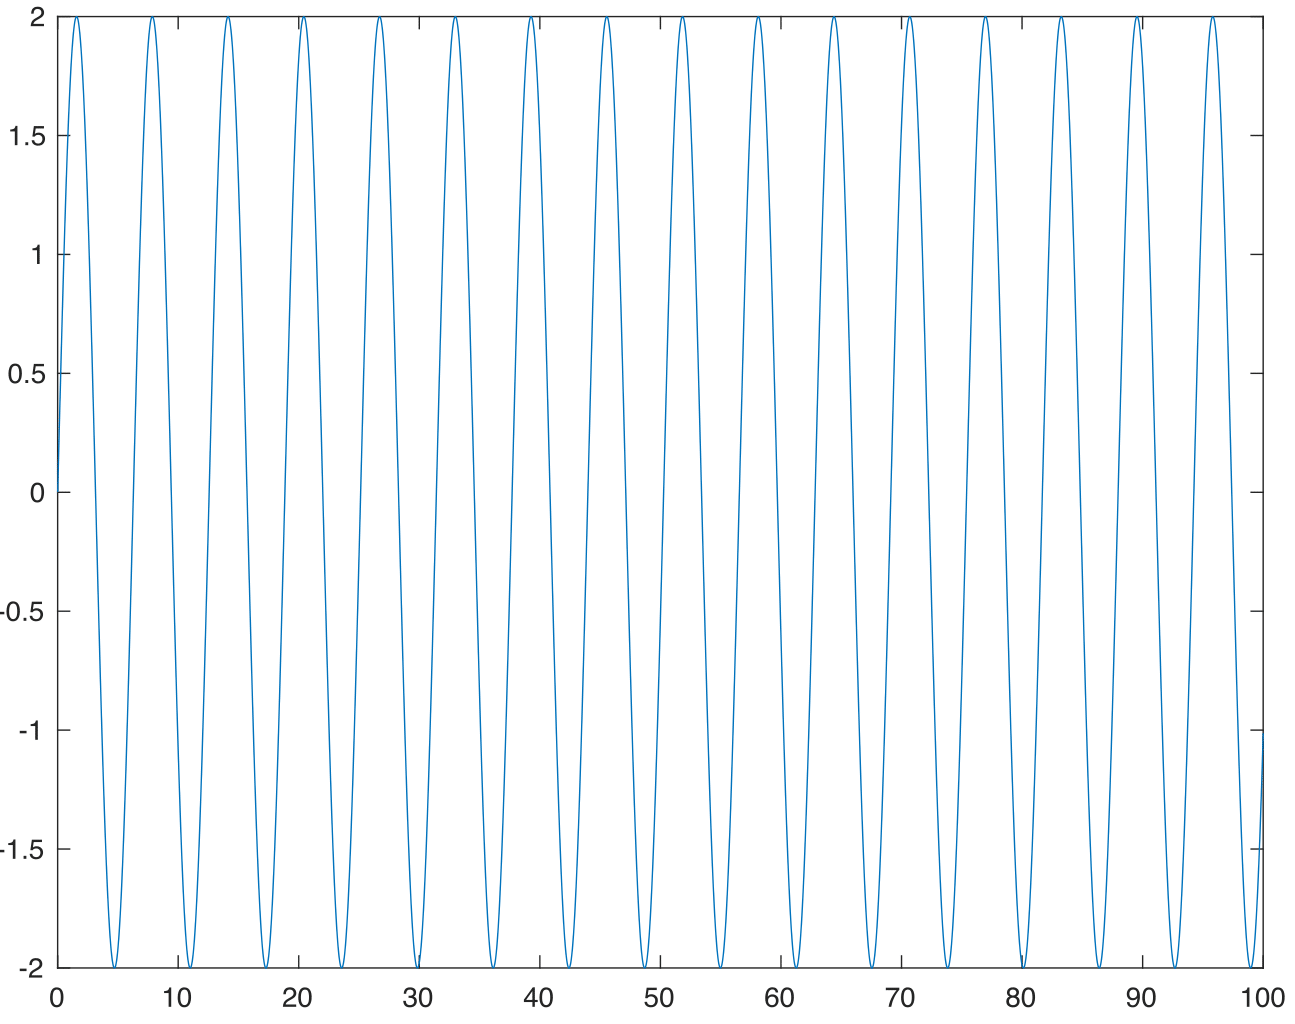
\includegraphics[width=0.5\textwidth]{Manual/Model1.png}
\end{figure}

\noindent The second model generates a sine wave with amplitude $0.5$ and frequency $1$ $rad/s$ that is represented in Figure~3.

\begin{figure}[h]
\caption{The signal $e$ generated from the model Model 2.}
  \centering
    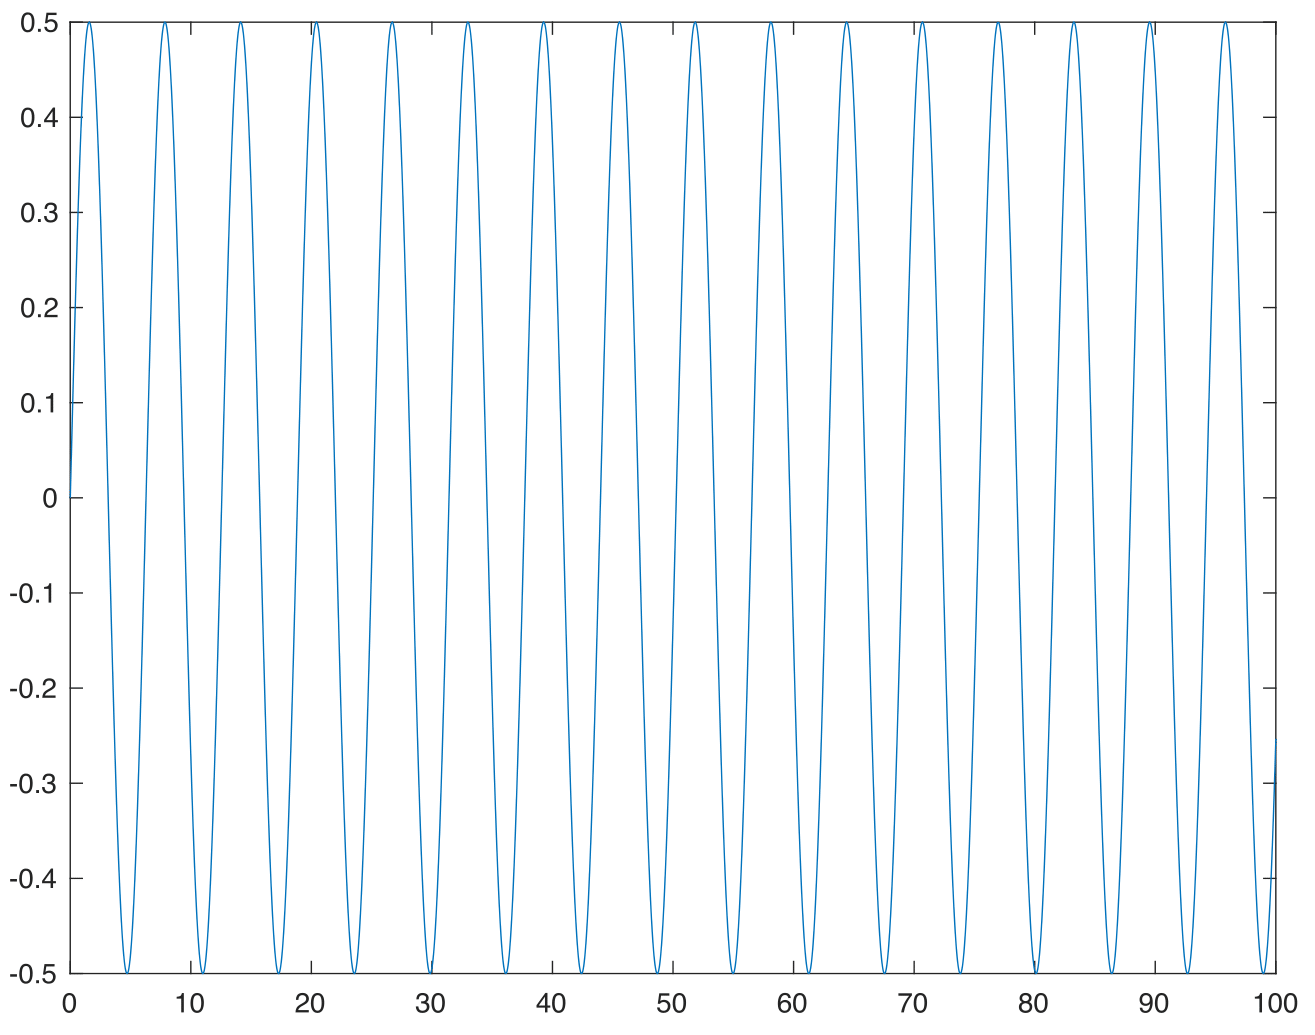
\includegraphics[width=0.5\textwidth]{Manual/Model2.png}
\end{figure}

\subsection{The Considered Requirements}
The first requirement (Test$\_$Forall) specifies that always the signal $e$ should not exceed the value $1$.
The requirement  Test$\_$Forall is reported in Figure~4.

\begin{figure}[h]
\caption{The requirement Test$\_$Forall.}
  \centering
    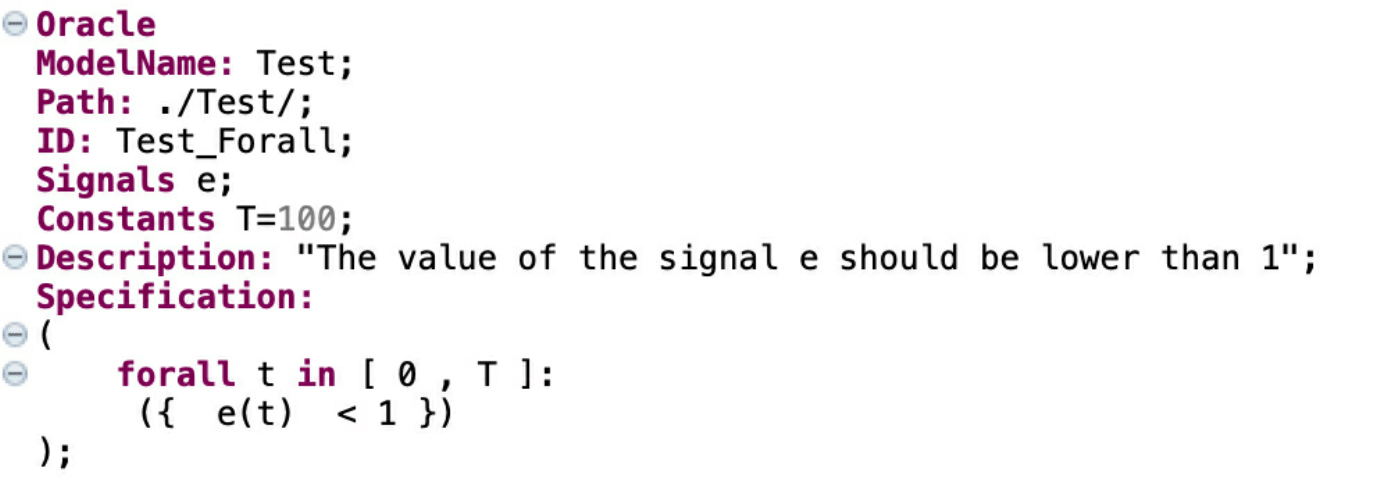
\includegraphics[width=0.8\textwidth]{Req1.png}
\end{figure}

\noindent The second requirement (Test$\_$Exists) specifies that there exists a time instant in which the signal $e$  exceeds the value $1$.
The requirement  Test$\_$Exists is reported in Figure~5.

\begin{figure}[h]
\caption{The requirement  Test$\_$Exists.}
  \centering
    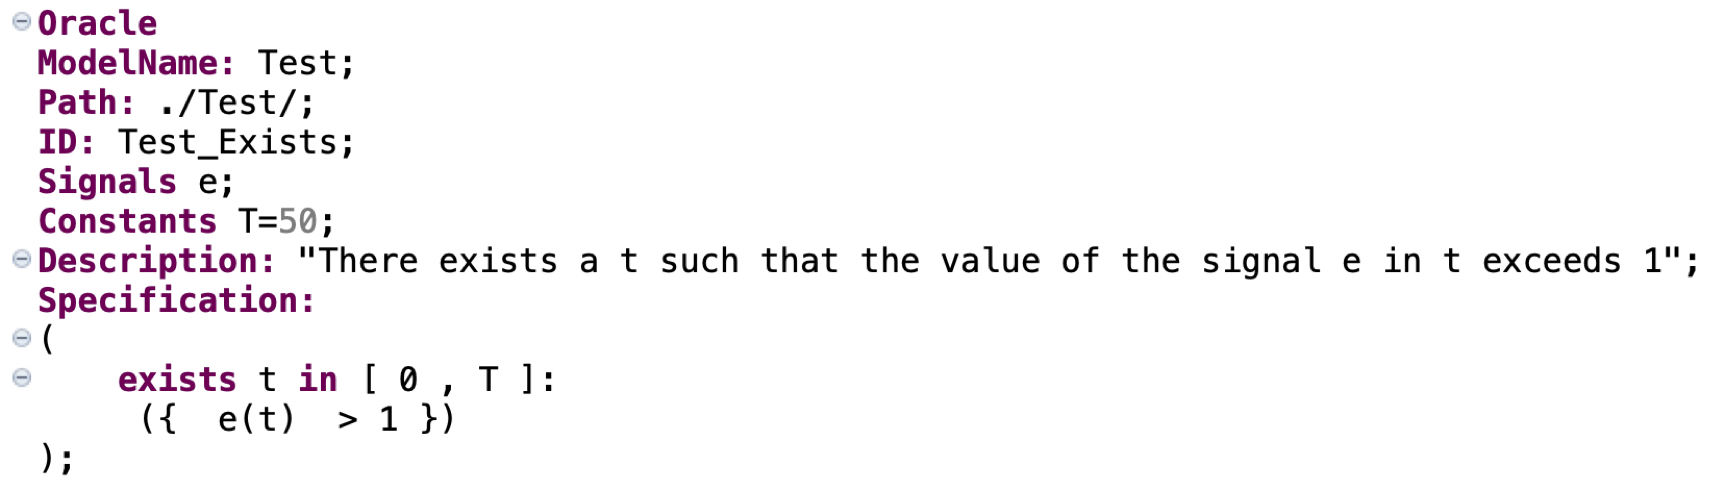
\includegraphics[width=0.95\textwidth]{Req2.png}
\end{figure}

\clearpage

\subsection{Scenario 1}
In scenario 1 the model Model 1 and the requirement Test$\_$Forall are considered. 
The evaluation of the oracle over time is presented in Figure~6.

\begin{figure}[h]
\caption{The evaluation of the oracle for the requirement Test$\_$Forall  and the model Model~1.}
  \centering
    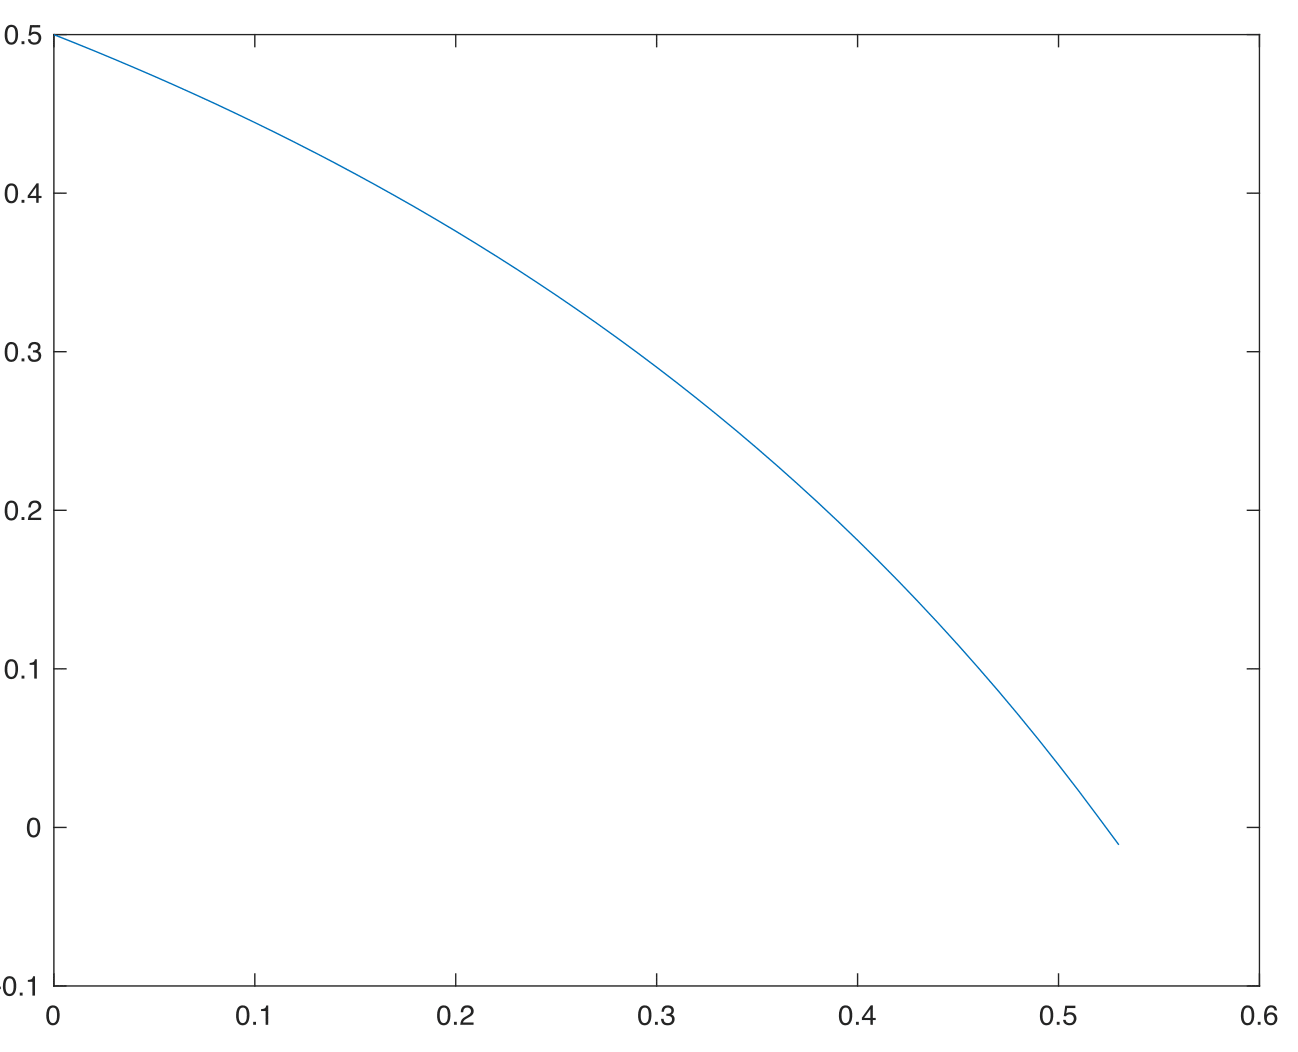
\includegraphics[width=0.5\textwidth]{resModel1TestForall.png}
\end{figure}


The oracle stops as soon as the requirement is detected to be violated.
The variable  $result\_Test\_Forall.Data$  contains the final result that for this simulation is: $-0.0109$.
Note that the result is negative. 
The property is indeed violated.

\subsection{Scenario 2}
In scenario 2 the model Model 2 and the requirement Test$\_$Forall are considered. 
The evaluation of the oracle over time is presented in Figure~7.

\begin{figure}[h]
\caption{The evaluation of the oracle for the requirement Test$\_$Forall  and the model Model~2.}
  \centering
    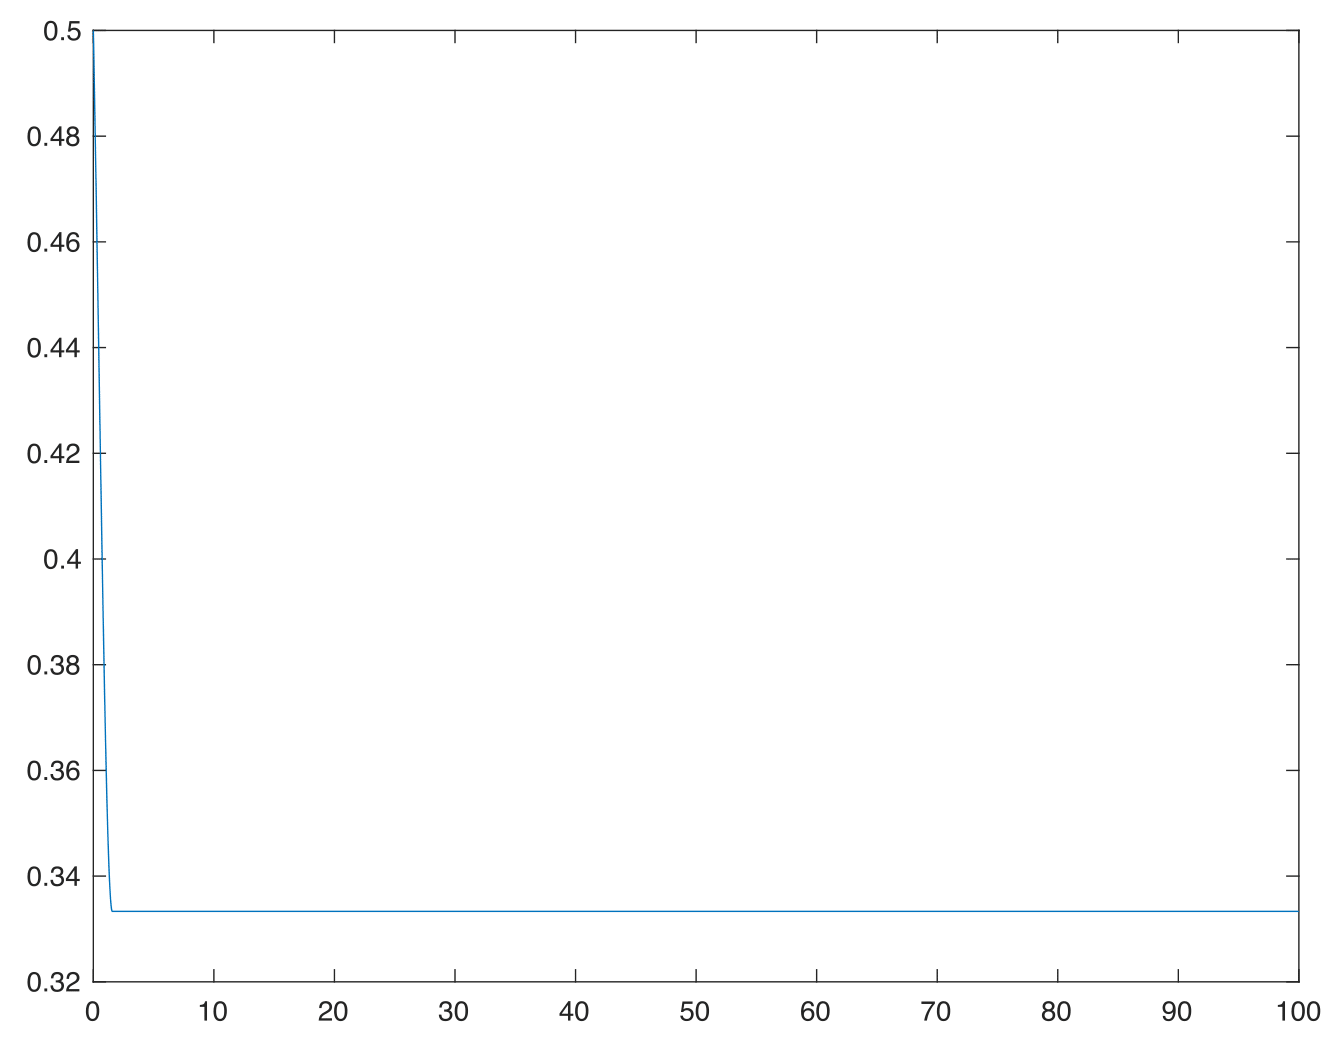
\includegraphics[width=0.5\textwidth]{resModel2TestForall.png}
\end{figure}

The variable $result\_Test\_Forall.Data$ contains the final result that for this simulation is: $0.3333$.
Note that the result is positive.
The property is indeed satisfied.


\subsection{Scenario 3}

\subsection{Scenario 4}

\end{document}